
\documentclass[article]{IEEEtran}
\usepackage[a5paper, margin=10mm, onecolumn]{geometry}

\usepackage{tfrupee} 
\setlength{\headheight}{1cm} 
\setlength{\headsep}{0mm}       
\usepackage{multicol}
\usepackage{gvv-book}
\usepackage{gvv}
\usepackage{cite}
\usepackage{amsmath,amssymb,amsfonts,amsthm}
\usepackage{algorithmic}
\usepackage{graphicx}
\usepackage{textcomp}
\usepackage{xcolor}
\usepackage{txfonts}
\usepackage{listings}
\usepackage{enumitem}
\usepackage{mathtools}
\usepackage{gensymb}
\usepackage{comment}
\usepackage[breaklinks=true]{hyperref}
\usepackage{tkz-euclide} 
\usepackage{listings}

\def\inputGnumericTable{}                                 
\usepackage[latin1]{inputenc}                                
\usepackage{color}                                            
\usepackage{array}                                            
\usepackage{longtable}                                       
\usepackage{calc}                                             
\usepackage{multirow}                                         
\usepackage{hhline}                                           
\usepackage{ifthen}                                           
\usepackage{lscape}
\begin{document}
	\title{8.2.20}
	\author{EE25BTECH11052 - Shriyansh Kalpesh Chawda}
	\maketitle
\textbf{Question}\\
 Find the equation of the conic, that satisfies the given
 conditions:\\
Vertex (0,0) passing through (2,3) and axis is along X axis.
\textbf{Solution}\\
The general conic is 
\begin{align}
 g(\vec{x}) = \vec{x}^\top \vec{V}\vec{x} + 2\vec{u}^\top \vec{x} + f = 0
\end{align}
\text{For axis along the $x$-axis, } 
\begin{align}
	\vec{V} = \myvec{A & 0 \\ 0 & C}, \quad 
	\vec{u} = \myvec{D \\ 0}
\end{align}
\text{Since the vertex is at the origin, } 
\begin{align}
\nabla g(\vec{0}) = 2\vec{u} = \vec{0} 
	\implies \vec{u} = \myvec{0 \\ 0}
\end{align}
If $ \det(\vec{V}) = AC \neq 0,$ then the conic has a center at the origin, which corresponds to an ellipse or hyperbola.\\
But the problem specifies a single vertex at the origin, not a center, so this case is invalid.


\begin{align}
	\therefore \det(\vec{V}) = 0 \quad \implies \quad \text{The conic is a parabola.}
\end{align}
\begin{align}
	g(\vec{x}) &= \vec{x}^\top \vec{V}\vec{x} + 2\vec{u}^\top \vec{x} + f = 0 
\end{align}
For a parabola with axis along the $x$-axis, vertex at origin,  
focus $\vec{F} = \myvec{p \\ 0}$ and directrix $\vec{n}^\top \vec{x} = c$,  
we have $\vec{n} = \myvec{1 \\ 0}, \; c = -p$.

\begin{align}
	\vec{V} &= \|\vec{n}\|^2 \vec{I} - \vec{n}\vec{n}^\top 
	= \myvec{1 & 0 \\ 0 & 1} - \myvec{1 \\ 0}\myvec{1 & 0} 
	= \myvec{0 & 0 \\ 0 & 1}
\end{align}

\begin{align}
	\vec{u} &= c\vec{n} - \vec{F} 
	= (-p)\myvec{1 \\ 0} - \myvec{p \\ 0} 
	= \myvec{-2p \\ 0}
\end{align}

\begin{align}
	f &= \|\vec{F}\|^2 - c^2 = p^2 - (-p)^2 = 0
\end{align}
Thus, the parabola equation becomes:
\begin{align}
	&\vec{x}^\top \myvec{0 & 0 \\ 0 & 1}\vec{x} 
	+ 2\myvec{-2p & 0}\vec{x} + 0 = 0\\
	&y^2 - 4px = 0
\end{align}
Since $(2,3)$ lies on the parabola:
\begin{align}
	3^2 - 4p(2) &= 0 \\
	9 - 8p &= 0 \\
	p &= \frac{9}{8}
\end{align}
Therefore,
\begin{align}
	\vec{V} &= \myvec{0 & 0 \\ 0 & 1}, \quad
	\vec{u} = \myvec{-\tfrac{9}{4} \\ 0}, \quad
	f = 0
\end{align}
and the equation of the required parabola is
\begin{align}
	y^2 = \frac{9}{2}x
\end{align}
\begin{figure}[H]
	\centering
	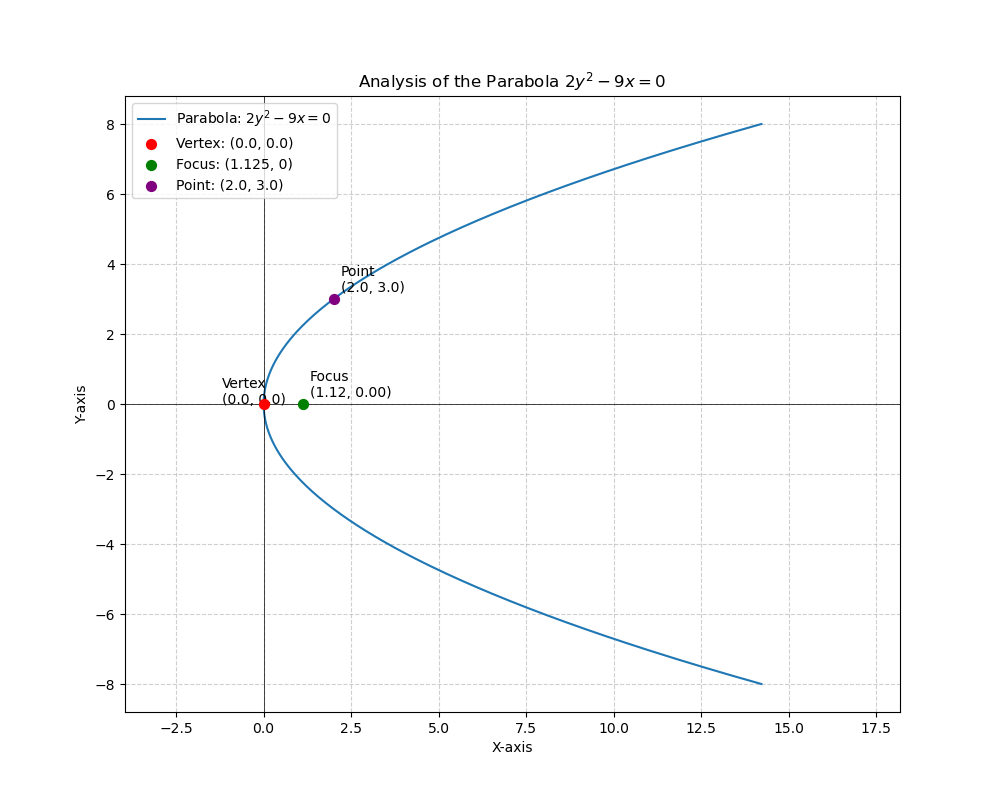
\includegraphics[width=1.\linewidth]{figs/parabola}

\end{figure}

	
\end{document}